\documentclass[10pt,tgadventor, onlymath]{beamer}

\usepackage{graphicx,amsmath,amssymb,tikz,psfrag,neuralnetwork}
\usepackage{xcolor}

\usetikzlibrary{positioning}

\input defs.tex
\graphicspath{ {./graphics/} }

%% formatting

\mode<presentation>
{
\usetheme{default}
\usecolortheme{seahorse}
}
\setbeamertemplate{navigation symbols}{}
\usecolortheme[rgb={0.03,0.28,0.59}]{structure}
\setbeamertemplate{itemize subitem}{--}
\setbeamertemplate{frametitle} {
	\begin{center}
	  {\large\bf \insertframetitle}
	\end{center}
}

\newcommand\footlineon{
  \setbeamertemplate{footline} {
    \begin{beamercolorbox}[ht=2.5ex,dp=1.125ex,leftskip=.8cm,rightskip=.6cm]{structure}
      \footnotesize \insertsection
      \hfill
      {\insertframenumber}
    \end{beamercolorbox}
    \vskip 0.45cm
  }
}
\footlineon

\AtBeginSection[] 
{ 
	\begin{frame}<beamer> 
		\frametitle{Outline} 
		\tableofcontents[currentsection, currentsubsection]
	\end{frame} 
} 


\tikzstyle{process} = [rectangle, minimum width=3cm, minimum height=1cm, text centered, draw=black]
\tikzstyle{arrow} = [thick,->,>=stealth]

\tikzstyle{state}=[shape=circle,draw=blue!30,fill=blue!10]
\tikzstyle{observation}=[shape=rectangle,draw=orange!30,fill=orange!10]
\tikzstyle{lightedge}=[<-, dashed]
\tikzstyle{mainstate}=[state, thick]
\tikzstyle{mainedge}=[<-, thick]
\tikzstyle{block} = [draw,rectangle,thick,minimum height=2em,minimum width=2em]
\tikzstyle{sum} = [draw,circle,inner sep=0mm,minimum size=2mm]
\tikzstyle{connector} = [->,thick]
\tikzstyle{line} = [thick]
\tikzstyle{branch} = [circle,inner sep=0pt,minimum size=1mm,fill=black,draw=black]
\tikzstyle{guide} = []
\tikzstyle{snakeline} = [connector, decorate, decoration={pre length=0.2cm,
                         post length=0.2cm, snake, amplitude=.4mm,
                         segment length=2mm},thick, magenta, ->]



%% begin presentation

\title{\large \bfseries Estimation of Channel Distribution Functions using a Neural Network}

\author{Peter Hartig\\[3ex]
}

\date{\today}

\begin{document}

\frame{
\thispagestyle{empty}
\titlepage
}

\frame{
\tableofcontents
}

\section{The channel state perspective}

\begin{frame}
\frametitle{The Channel State}
\begin{itemize}
\item 
	Observations are made of some channel in a point-to-point communication system.
\item 
	For each observation, this channel takes on a state $s[k]\in \cal{S}$. 
\item 
	The true state $s[k]$ is hidden by the addition of noise to an observation $y[k]$.
\end{itemize}
\end{frame}
\begin{frame}

\frametitle{Sampling Channel State}
Over many observations, the sequence $\mathbf{y}$ corresponds to a sequence of channel states $\mathbf{s}\in\textit{\cal{S}}^N$
\begin{figure}[H]
\begin{center}
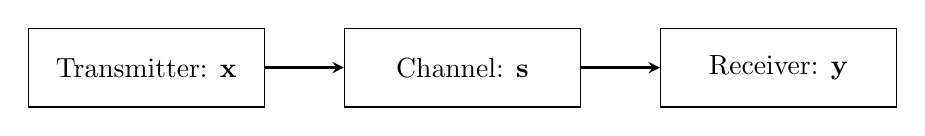
\begin{tikzpicture}[node distance=1cm]
\node (transmitter) [process] {Transmitter: $\mathbf{x}$};
\node (channel) [process, right = of transmitter] {Channel: $\mathbf{s}$};
\node (receiver) [process, right = of channel] {Receiver: $\mathbf{y}$};
\draw [arrow] (transmitter) -- (channel);
\draw [arrow] (channel) -- (receiver);
\end{tikzpicture}
\end{center}
\end{figure}
\pause
For a channel represented by an LTI system, the state is determined entirely by the transmitted information $\mathbf{x}$.
\end{frame}

\begin{frame}
\frametitle{Estimating the True Channel State}
\begin{block}{Goal:}
We attempt to estimate the true, hidden, sequence of channel states, $\mathbf{s}$, based the sequence of samples $\mathbf{y}$.
\end{block}

\begin{block}{Note}
Assume we known the number of channel states $|\textit{\cal{S}}|$
\end{block}

\end{frame}
\section{The optimization framework}

\begin{frame}
\frametitle{MAP Sequence Detection}
\begin{equation*}
\underset{\mathbf{s}\in\textcolor{red}{\textit{\cal{S}}^N}}{\text{maximize}} \; p(\mathbf{s}|\mathbf{y}).
\end{equation*} 
\pause
Using Bayes' theorem
\begin{equation*}
p(\mathbf{s}|\mathbf{y}) = 
\frac
{p(\mathbf{y}|\mathbf{s})p(\mathbf{s})}
{p(\mathbf{y})}
\end{equation*} 
Noting that $p(\mathbf{y})$ can be ignored 
\pause
\begin{equation}\label{opt_problem}
\underset{\mathbf{s}\in\textit{\cal{S}}^N}{\text{maximize}}\; p(\mathbf{y}|\mathbf{s})p(\mathbf{s})
\end{equation}

\end{frame}

\begin{frame}
\frametitle{MAP Sequence Detection}
\begin{equation*}\label{opt_problem}
\underset{\mathbf{s}\in\textit{\cal{S}}^N}{\text{maximize}}\; p(\mathbf{y}|\mathbf{s})p(\mathbf{s})
\end{equation*}
\pause
Assuming 
\begin{equation*}
p(\mathbf{y}|\mathbf{s}) = \prod_{k=0}^{N-1} p(y[k]|\mathbf{s})
\end{equation*}
\pause
and 
\begin{equation*}
p(y[k]|\mathbf{s}) = p(y[k]|s[k])
\end{equation*}
\pause
this simplifies to 
\begin{equation*}\label{opt_problem}
\underset{\mathbf{s}\in\textit{\cal{S}}^N}{\text{maximize}}\; \prod_{k=0}^{N-1} p(y[k]|s[k])p(\mathbf{s}).
\end{equation*}
\end{frame}

\begin{frame}
\frametitle{MAP Sequence Detection}
For the LTI channel
\begin{gather*}
p(\mathbf{s}) \\=\\
 p(s[N]| s[N-1]... \; s[0]) p(s[N-1]| s[N-2]... \; s[0])... \; p(s[1]| s[0])p(s[0])
\end{gather*}
describes the consistency of transmitted symbols implied by the state sequence.
The channel states of the LTI channel satisfy the Markov property 
\begin{gather*}
 p(s[N]| s[N-1]... \; s[0]) =  p(s[N]| s[N-1]]).
\end{gather*}

\end{frame}

\begin{frame}
\frametitle{Example with LTI channel - Continued}
With these assumptions,
\begin{equation*}\label{opt_problem}
\underset{\mathbf{s}\in\textit{\cal{S}}^N}{\text{maximize}}\; \prod_{k=0}^{N-1} p(y[k]|s[k])p(\mathbf{s})
\end{equation*}
 is equivalent to  
\begin{equation*}\label{opt_problem}
\underset{\mathbf{s}\in\textit{\cal{S}}^N}{\text{minimize}}\; \sum_{k=0}^{N-1} -log(p(y[k]|s[k])p(s[k]|s[k-1])).
\end{equation*}
For the LTI channel $p(s[k]|s[k-1])$ is 0 if states contradict transmission sequence, otherwise this term is constant.
\end{frame}


\begin{frame}
\frametitle{Viterbi Algorithm}
\begin{equation*}\label{opt_problem}
\underset{\mathbf{s}\in\textit{\cal{S}}^N}{\text{minimize}}\; \sum_{k=0}^{N-1} -log(p(y[k]|s[k])p(s[k]|s[k-1])).
\end{equation*}
    \noindent\rule[10pt]{\textwidth}{0.4pt}
	\begin{center}
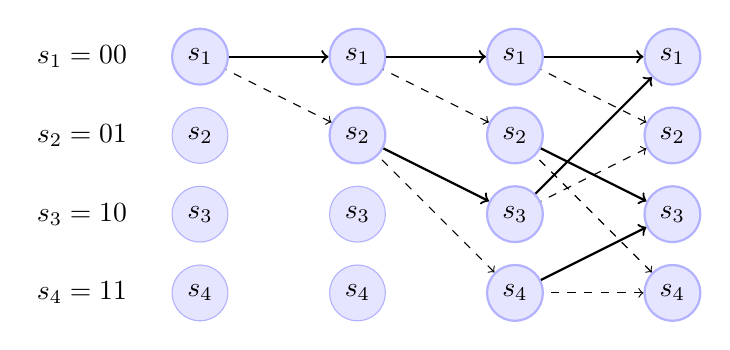
\begin{tikzpicture}[]
% 1st column
\node               at (-1.5,5) {$s_1=00$};
\node               at (-1.5,4) {$s_2=01$};
\node               at (-1.5,3) {$s_3=10$};
\node               at (-1.5,2) {$s_4=11$};
\node[mainstate] (s1_1) at (0,5) {$s_1$};
\node[state] (s2_1) at (0,4) {$s_2$};
\node[state] (s3_1) at (0,3) {$s_3$};
\node[state] (s4_1) at (0,2) {$s_4$};
%\node at (0,1) {Node1};
% 2nd column
\node[mainstate] (s1_2) at (2,5) {$s_1$}
    edge[mainedge] (s1_1);
\node[mainstate] (s2_2) at (2,4) {$s_2$}
     edge[lightedge] (s1_1);

\node[state] (s3_2) at (2,3) {$s_3$};

\node[state] (s4_2) at (2,2) {$s_4$};

%\node at (2,1) {Node2};
% 3rd column
%\node               at (4,6) {$t=2$};
\node[mainstate] (s1_3) at (4,5) {$s_1$}
    edge[mainedge]  (s1_2);

\node[mainstate] (s2_3) at (4,4) {$s_2$}
    edge[lightedge] (s1_2);

\node[mainstate] (s3_3) at (4,3) {$s_3$}
    edge[mainedge] (s2_2);    
\node[mainstate] (s4_3) at (4,2) {$s_4$}
    edge[lightedge] (s2_2);
%\node at (4,1) {Node3};
% 4th column
%\node               at (6,6) {$t=3$};
\node[mainstate] (s1_4) at (6,5) {$s_1$}
    edge[mainedge]  (s1_3)
    edge[mainedge]  (s3_3);
\node[mainstate] (s2_4) at (6,4) {$s_2$}
    edge[lightedge] (s1_3)
    edge[lightedge] (s3_3);
\node[mainstate] (s3_4) at (6,3) {$s_3$}
    edge[mainedge] (s2_3)
    edge[mainedge] (s4_3);
\node[mainstate] (s4_4) at (6,2) {$s_4$}
    edge[lightedge] (s2_3)
    edge[lightedge] (s4_3);
%\node at (6,1) {Node4};

\end{tikzpicture}
	\end{center}
			Example with channel impulse response length 2 and constellation size 2.

\end{frame}

\section{Incorporating a Neural Network}

\begin{frame}
\frametitle{Decomposing Terms in the Viterbi Algorithm}
The individual terms in
\begin{equation*}\label{opt_problem}
\underset{\mathbf{s}\in\textit{\cal{S}}^N}{\text{minimize}}\; \sum_{k=0}^{N-1} -log(p(y[k]|s[k])p(s[k]|s[k-1])).
\end{equation*}
can be rewritten 
\begin{equation*}
p(y[k]|s[k])p(s[k]|s[k-1]) = \frac{p(s[k]|y[k])p(y[k])}{p(s[k])}p(s[k]|s[k-1]).
\end{equation*}
\end{frame}

\begin{frame}
	\frametitle{Decomposing Terms in the Viterbi Algorithm}
\begin{equation*}
\frac{\textcolor{red}{p(s[k]|y[k])}p(y[k])}{p(s[k])}
\end{equation*}
\begin{figure}[H]
		\centering
		\begin{neuralnetwork}[height=3, nodespacing=15mm, layerspacing=26mm]
		\newcommand{\x}[2]{$y[\text{k}]$}
		\newcommand{\y}[2]{$p(s_{#2}[\text{k}]|y[\text{k}])$}
		\newcommand{\hfirst}[2]{ $h^{(1)}_#2$}
		\newcommand{\hsecond}[2]{ $h^{(2)}_#2$}
		\newcommand{\hthird}[2]{$h^{(3)}_#2$}
		\newcommand{\hfourth}[2]{$h^{(4)}_#2$}
		\inputlayer[count=1, bias=false, title=\\, text=\x]
		\hiddenlayer[count=2, bias=false, title=\\, text=\hthird] \linklayers
		\hiddenlayer[count=3, bias=false, title=\\, text=\hfourth] \linklayers
		\outputlayer[count=4, title=\\, text=\y] \linklayers
	    \end{neuralnetwork}

\label{nn}

\end{figure}
\end{frame}

\begin{frame}
	\frametitle{Decomposing Terms in the Viterbi Algorithm }
\begin{equation*}
\frac{p(s[k]|y[k])\textcolor{red}{p(y[k])}}{p(s[k])}
\end{equation*}
\\
\begin{equation*}
p(y[k]) = \sum_{s_i \in \mathcal{S}} p(y[k],s_i)
\end{equation*}
\centering
	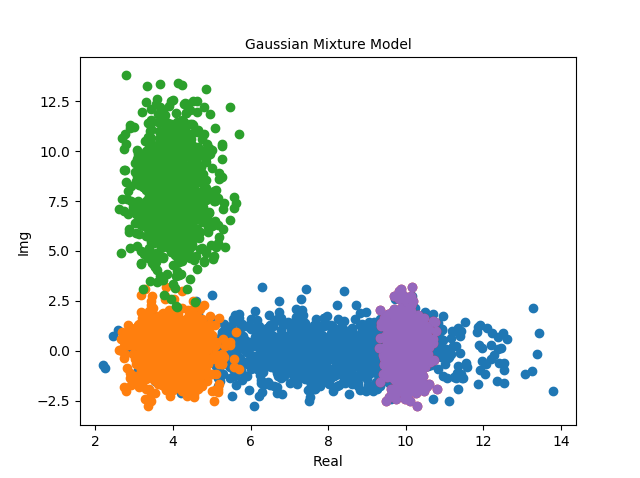
\includegraphics[width=8cm, height=5.5cm ]{system_model/mm}
\end{frame}

\begin{frame}
	\frametitle{Decomposing Terms in the Viterbi Algorithm}
\begin{equation*}
\frac{p(s[k]|y[k])p(y[k])}{\textcolor{red}{p(s[k])}}
\end{equation*}
\end{frame}



\section{Extension of ViterbiNet: Reduced}
\begin{frame}
	\frametitle{State Redundancy}
\begin{columns}
\begin{column}{0.5\linewidth}
\centering
\begin{figure}
	\includegraphics[width=\textwidth]{system_model/channel_output_2}
	\caption{AWGN channel output for CIR = $[1, .7, 0.4, 0.1]$ with SNR = $15$ dB}
\end{figure}
\end{column}
\begin{column}{0.5\linewidth}
\centering
\begin{figure}
	\includegraphics[width=\textwidth]{system_model/channel_output_1}
	\caption{AWGN channel output for CIR =  $[1, 1, 0.15, 0.1]$ with SNR = $15$ dB}
\end{figure}
\end{column}
\end{columns}

\end{frame}

\begin{frame}
	\frametitle{Exploiting State Redundancy}
\begin{enumerate}
\item Cluster some set of observed channel output into desired number of states
\pause
\item For states with ambiguous channel input, use majority decision
\pause
\item *Choosing too few states will degrade performance
\end{enumerate}
\end{frame}


\section{Simulation Results}
\begin{frame}
\frametitle{Simulation System}
\begin{itemize}
\item BPSK with AWGN at receiver with SNR given by 
\begin{equation*}
\text{SNR} = \frac{E\{|x[k]|^2\}}{E\{|n[k]|^2\}}
\end{equation*}
\item 
Impulse response is normalized. 
\end{itemize}
\end{frame}

\begin{frame}
\frametitle{Detection Performance: LTI Channel}
\begin{columns}
\begin{column}{0.5\linewidth}
\centering
CIR = $[0.9, 0.7, 0.3, 0.5, 0.1]$
	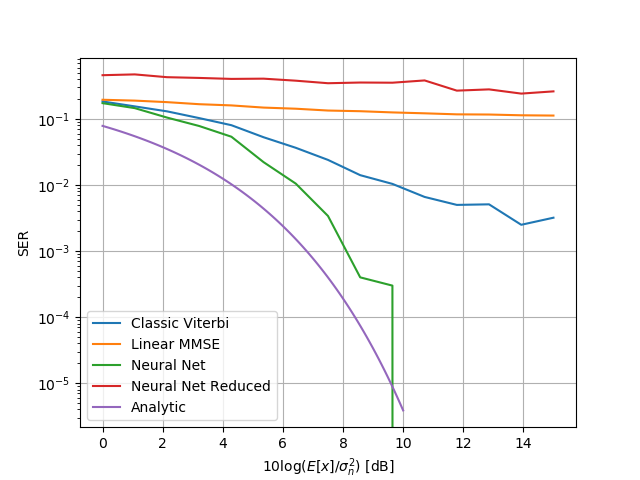
\includegraphics[width=\textwidth]{results/lti_32_reduced_asymmetric}
\end{column}
\begin{column}{0.5\linewidth}
\centering
CIR = $[.9, 0, .0, .4, .7]$
	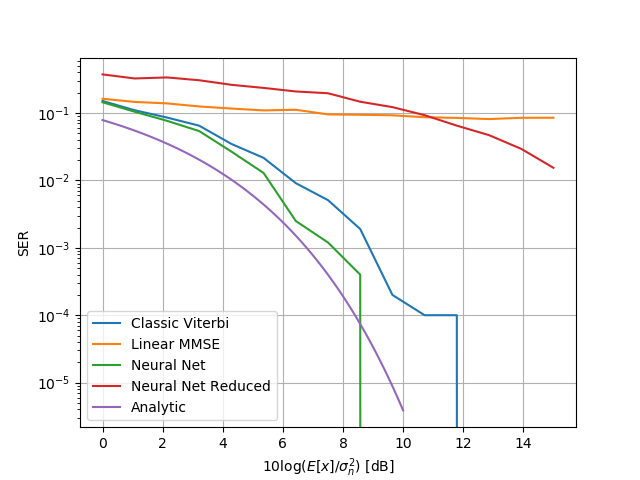
\includegraphics[width=\textwidth]{results/lti_8_reduced}
\end{column}
\end{columns}
*Reduced states uses 8 states in both figures above
\end{frame}
\begin{frame}
\frametitle{Detection Performance: Quantizer}
\begin{figure}
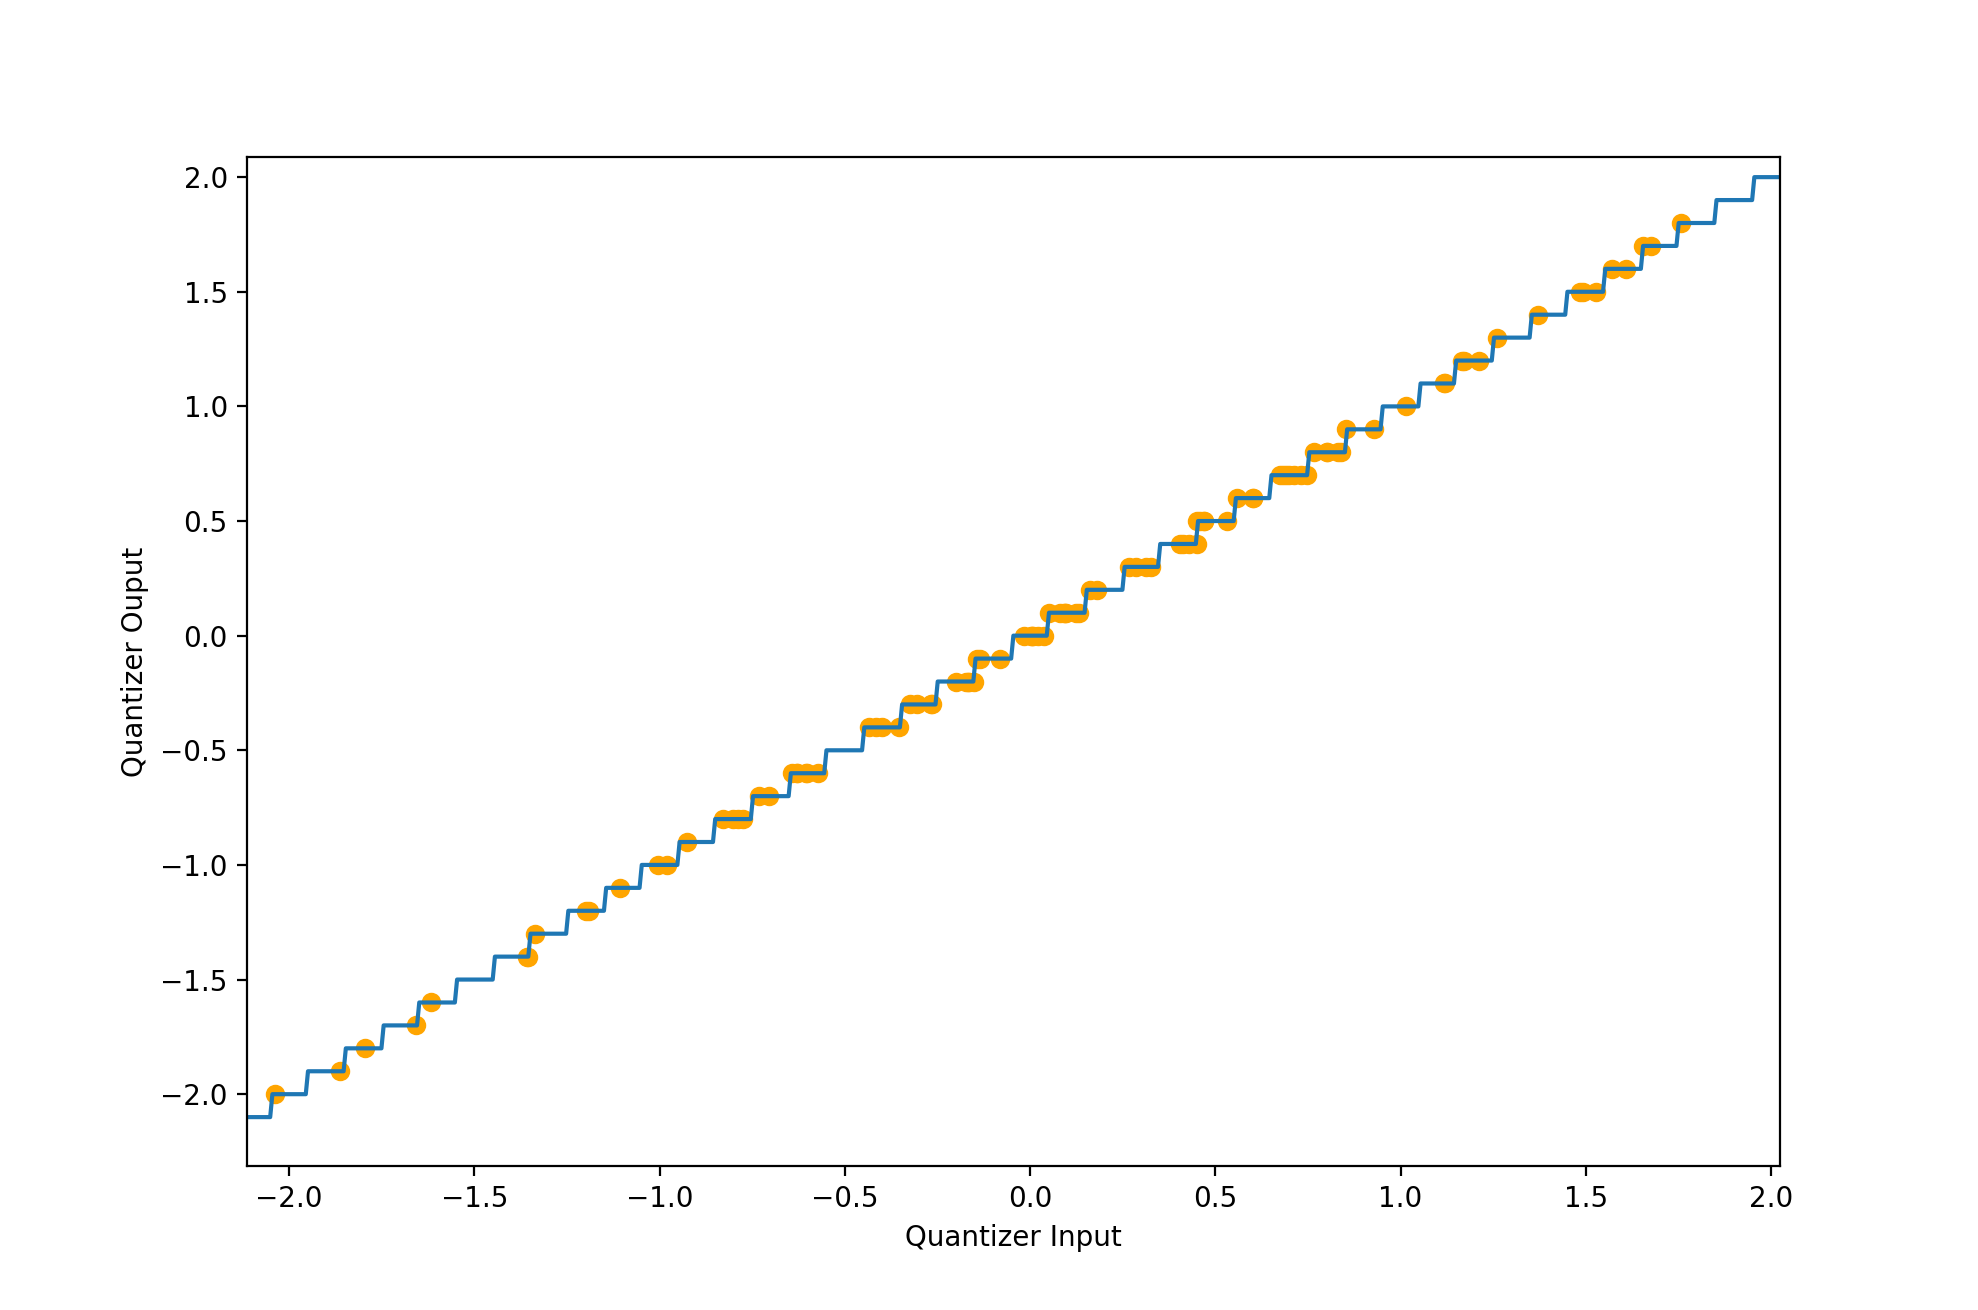
\includegraphics[width= 8cm, height = 5cm]{system_model/quantizer_overlay_new}
	\caption{Quantizer input/output for AWGN channel with CIR = $[ 0.9, 0.7, 0.3, 0.5, 0.1]$ (32 states) with SNR = $10$ dB}
\end{figure}
Implementated by rounding down to chosen number of decimal places \emph{after} adding noise at receiver. 
\end{frame}

\begin{frame}
\frametitle{Detection Performance: LTI Channel with Quantization}
\begin{columns}
\begin{column}{0.5\linewidth}
\centering
CIR = $[0.9, 0.7, 0.3, 0.5, 0.1]$
	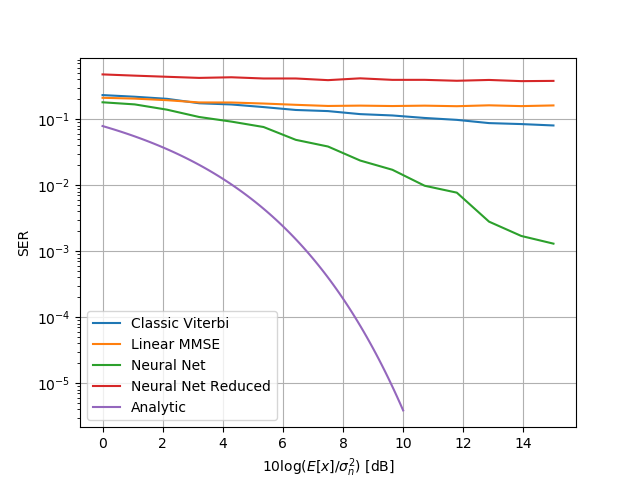
\includegraphics[width=\textwidth]{results/lti_32_reduced_asymmetric_quantized}
\end{column}
\begin{column}{0.5\linewidth}
\centering
CIR = $[.9, 0, .0, .4, .7]$
	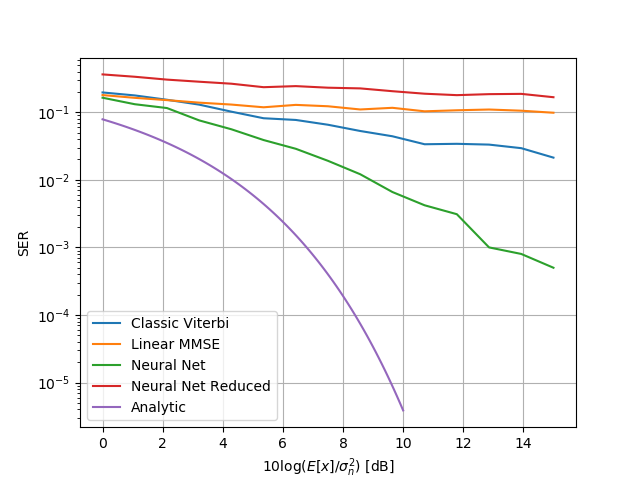
\includegraphics[width=\textwidth]{results/lti_8_reduced_quantized}
\end{column}
\end{columns}

*Reduced states uses 8 states in both figures above
\\
*Note that the "Classic" Viterbi is no longer using ideal metric here
\end{frame}

\section{Conclusion}

\begin{frame}
\frametitle{Other Notes}
\begin{itemize}
\item Can be applied to other algorithms (BCJR).
\item Generate training data for molecular communications channel and test on real data.
\end{itemize}
\end{frame}

\begin{frame}
  \centering \Large
  \emph{Thank You.}
  \\
	\bigskip
    \centering \Large
  \emph{Questions or Comments?}
\end{frame}
\end{document}
